\documentclass{article}%
\usepackage[T1]{fontenc}%
\usepackage[utf8]{inputenc}%
\usepackage{lmodern}%
\usepackage{textcomp}%
\usepackage{lastpage}%
\usepackage[head=40pt,margin=0.5in,bottom=0.6in]{geometry}%
\usepackage{graphicx}%
%
\title{\textbf{ONU aprobó resolución sobre la crisis humanitaria en Venezuela}}%
\author{El Nacional Web | Con información de EFE}%
\date{27/09/2018}%
%
\begin{document}%
\normalsize%
\maketitle%
\textbf{URL: }%
http://www.el{-}nacional.com/noticias/mundo/onu{-}aprobo{-}resolucion{-}sobre{-}crisis{-}humanitaria{-}venezuela\_253427\newline%
%
\textbf{Periodico: }%
EN, %
ID: %
253427, %
Seccion: %
Mundo\newline%
%
\textbf{Palabras Claves: }%
Mundo, Crisis humanitaria, ONU\newline%
%
\textbf{Derecho: }%
18, %
Otros Derechos: %
5, %
Sub Derechos: %
\newline%
%
\textbf{EP: }%
NO\newline%
\newline%
%
\textbf{\textit{El informe insta al gobierno de Nicolás Maduro a que acepte ayuda humanitaria y coopere con la Oficina del Alto Comisionado y los mecanismos del Consejo de Derechos Humanos de la organización~}}%
\newline%
\newline%
%
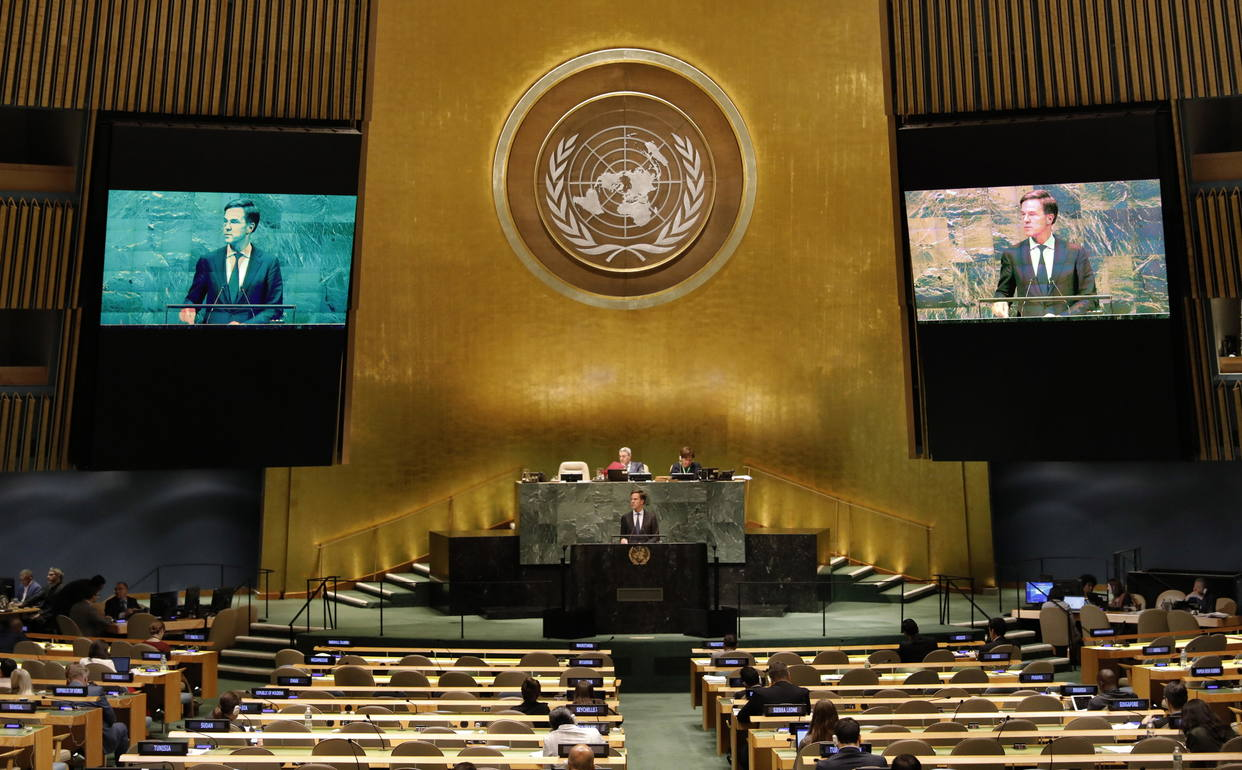
\includegraphics[width=300px]{233.jpg}%
\newline%
%
El Consejo de Derechos Humanos de la Organización de las Naciones Unidas (ONU) aprobó la mañana de este miércoles la~resolución sobre la crisis humanitaria que atraviesa Venezuela.%
\newline%
%
La medida, que contó con 23 votos a favor, 7 en contra y 17 abstenciones, exhorta al gobierno de Nicolás Maduro a que acepte la ayuda humanitaria para paliar la escasez de alimentos, medicinas y suministros médicos que hay en el país.%
\newline%
%
Además, insta al gobierno venezolano a que coopere con la Oficina del Alto Comisionado y los mecanismos del Consejo de Derechos Humanos de la organización.%
\newline%
%
De la misma forma, solicita a la alta comisionada de la ONU para derechos humanos, Michelle Bachelet, que prepare un nuevo informe exhaustivo sobre la situación en~Venezuela~y que se lo presente en junio de 2019. Para su sesión de inicios del próximo marzo, le encarga que exponga oralmente información actualizada sobre ese tema.%
\newline%
%
La medida adoptada también hace mención de la preocupación~de los países por las violaciones de los derechos humanos en el contexto de la crisis política, económica, social y humanitaria de Venezuela.%
\newline%
%
Afganistán, Australia, Bélgica, Brasil, Chile, Croacia, Ecuador, Georgia, Alemania, Hungría, Islandia, Japón, México, Panamá, Perú, Corea del Sur, Ruanda, Eslovaquia, Eslovenia, España, Suiza, Ucrania y el Reino Unido fueron los países que aceptaron la medida.%
\newline%
%
Por otro lado, Burundi, China, Cuba, Egipto, Pakistán, Venezuela y la República democrática del Congo rechazaron la resolución.%
\newline%
%
El embajador de Perú, Claudio de la Puente, dijo que llegó el momento de que el Consejo atienda a la situación que ha provocado el éxodo de millones de venezolanos.%
\newline%
%
Por otro lado, el representante venezolano ante la ONU en Ginebra, Jorge Valero, condenó la medida y la consideró como “el comienzo de una escalada intervencionista" para conseguir la caída del gobierno de Maduro. Además, acusó a los países que promovieron la resolución de ser instrumentos de Estados Unidos e Israel en contra de Venezuela.%
\newline%
%
Argentina, Chile, Colombia, Paraguay,~Perú y Canadá~se unieron este miércoles al margen de su participación en la Asamblea General de ONU en Nueva York para pedir formalmente a la Fiscalía de la Corte Penal Internacional~que investigue los crímenes de lesa humanidad en~Venezuela.%
\newline%
%
A continuación la resolución:%
\newline%
%
\end{document}